\section{Finite dimensional representations of \texorpdfstring{$\sll_2(k)$}{sl2(k)}}
Recall that the standard basis $(e,h,f)$ of $\sll_2(k)$ is given by
\[
 e = \begin{pmatrix} 0 & 1 \\ 0 & 0 \end{pmatrix}, \quad
 h = \begin{pmatrix} 1 & 0 \\ 0 & -1 \end{pmatrix}, \quad
 f = \begin{pmatrix} 0 & 0 \\ 1 & 0 \end{pmatrix}.
\]
This basis satisfies the relations
\[
 [h,e] = 2e, \quad
 [h,f] = -2f, \quad
 [e,f] = h.
\]


\begin{defi}
 Let $V$ be a representation of $\sll_2(k)$. For any $\lambda \in k$ let
 \[
  V_\lambda \coloneqq \{v \in V \mid h.v = \lambda v\}.
 \]
\end{defi}


\begin{lem}\label{lem: e and f moving the eigenspaces}
 Let $V$ a representation of $\g$ and $\lambda \in k$. Then
 \[
  e.V_\lambda \subseteq V_{\lambda+2}
  \quad\text{and}\quad
  f.V_\lambda \subseteq V_{\lambda-2}.
 \]
\end{lem}
\begin{proof}
 Let $v \in V_\lambda$. Then
 \begin{gather*}
  h.(e.v)
  = e.h.v + [h,e].v
  = \lambda e.v + 2e.v
  = (\lambda+2) e.v
 \shortintertext{and}
  h.(f.v)
  = h.f.v + [h,f].v
  = \lambda h.v - 2f.v
  = (\lambda-2) f.v.
 \qedhere
 \end{gather*}
\end{proof}


\begin{expl}\label{expl: natural representation of sl2}
 Let $e_1$, $e_2$ be the standard basis of $V \coloneqq k^2$, which is the natural representation of $\sll_2(k)$. Then $h.e_1 = e_1$ and $h.e_2 = -1$, so $V_1 = k e_1$ and $V_{-1} = k e_2$ with $V = V_{-1} \oplus V_1$. Then $e.V_{-1} = V_1$ and $f.V_1 = V_{-1}$.
\end{expl}


\begin{thrm}[Classification of finite dimensional irreducible representations of $\sll_2(k)$]
 For every $n \geq 1$ there exists up to isomorphism a unique $n$-dimensional irreducible representation of $\sll_2(k)$. More explicitely:
 \begin{enumerate}[leftmargin=*]
  \item
   For every $n \geq 1$ there exists an $n$-dimensional irreducible representation $V^{(n)}$ of $\sll_2(k)$.
  \item
   Let $V$ be an $n$-dimensional irreducible representation of $\sll_2(k)$ for some $n \geq 1$. Then
   \[
    V = V_{-n+1} \oplus V_{-n+3} \oplus \dotsb \oplus V_{n-3} \oplus V_{n-1}
   \]
   and $V_i$ is one-dimensional for every $i = -n+1, -n+3, \dotsc, n-3, n-1$.
   
   More explicitely there exists a basis $v_1, \dotsc, v_n$ of $V$ with $v_i \in V_{-n-1+2i}$ for every $i = 1, \dotsc, n$, with respect to which the actions of $e$ and $f$ are given as in the following diagram, where the dashed arrows represent the action of $f$.
   \begin{center}
    \tikzsetnextfilename{irreducible_representation_of_sl2}
    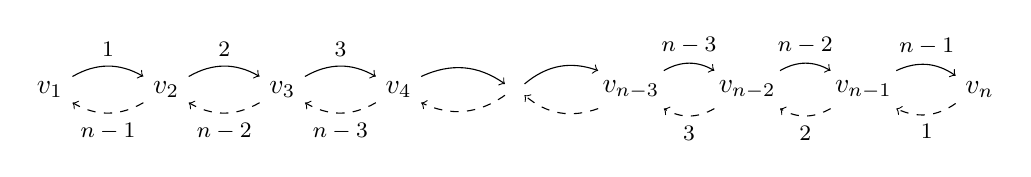
\begin{tikzpicture}[node distance = 4.2em]
     % the nodes
     \node (v1) {$v_1$};
     \node[right of = v1] (v2) {$v_2$};
     \node[right of = v2] (v3) {$v_3$};
     \node[right of = v3] (v4) {$v_4$};
     \node[right of = v4] (dots) {$\dotso$};
     \node[right of = dots] (vn-3) {$v_{n-3}$};
     \node[right of = vn-3] (vn-2) {$v_{n-2}$};
     \node[right of = vn-2] (vn-1) {$v_{n-1}$};
     \node[right of = vn-1] (vn) {$v_n$};
     % the action of e
     \draw[->, bend left] (v1) to node[above] {\footnotesize $1$} (v2);
     \draw[->, bend left] (v2) to node[above] {\footnotesize $2$} (v3);
     \draw[->, bend left] (v3) to node[above] {\footnotesize $3$} (v4);
     \draw[->, bend left] (v4) to (dots);
     \draw[->, bend left] (dots) to (vn-3);
     \draw[->, bend left] (vn-3) to node[above] {\footnotesize $n-3$} (vn-2);
     \draw[->, bend left] (vn-2) to node[above] {\footnotesize $n-2$} (vn-1);
     \draw[->, bend left] (vn-1) to node[above] {\footnotesize $n-1$} (vn);
     % the action of f
     \draw[->, bend left, dashed] (vn) to node[below] {\footnotesize $1$} (vn-1);
     \draw[->, bend left, dashed] (vn-1) to node[below] {\footnotesize $2$} (vn-2);
     \draw[->, bend left, dashed] (vn-2) to node[below] {\footnotesize $3$} (vn-3);
     \draw[->, bend left, dashed] (vn-3) to (dots);
     \draw[->, bend left, dashed] (dots) to (v4);
     \draw[->, bend left, dashed] (v4) to node[below] {\footnotesize $n-3$} (v3);
     \draw[->, bend left, dashed] (v3) to node[below] {\footnotesize $n-2$} (v2);
     \draw[->, bend left, dashed] (v2) to node[below] {\footnotesize $n-1$} (v1);
    \end{tikzpicture}
   \end{center}
   In particular
   \begin{gather*}
    e.V_i =
    \begin{cases}
     V_{i+2} & \text{for $i = -n+1, -n+3, \dotsc, n-3$}, \\
     0       & \text{otherwise},
    \end{cases}
   \shortintertext{and}
    f.V_i =
    \begin{cases}
     V_{i-2} & \text{if $i = -n+3, \dotsc, n-3, n-1$}, \\
     0       & \text{otherwise}.
    \end{cases}
   \end{gather*}
 \end{enumerate}
\end{thrm}
\begin{proof}
 \begin{enumerate}[leftmargin=*]
  \item
   Let $\sll_2(k)$ act on $V \coloneqq k[x,y]$ via
   \[
    \sll_2(k) \to \gl(V), \quad
    e \mapsto y\dd{x}, \quad
    h \mapsto y\dd{y}-x\dd{x}, \quad
    f \mapsto x\dd{y}.
   \]
   It was already shown in Examples~\ref{expls: representations of Lie algebras} that this defines a representation of $\sll_2(k)$. Let $V^{(n)} \subseteq V$ be the linear subspace consisting of the homogeneous polynomials of degree $n-1$, i.e.\
   \[
    V^{(n)} = \vspan_k\left( x^{n-1}, x^{n-2} y, \dotsc, x y^{n-2}, y^{n-1} \right).
   \]
   Then $V^{(n)}$ is an $n$-dimensional subrepresentation of $V$.
   
   Let $U \subseteq V^{(n)}$ be a nonzero subrepresentation. If $p \in U$ is a nonzero polynomial then by applying $f$ often enough it follows that $x^{n-1} \in U$, from which it follows from applying $e$ often enough that $x^{n-i} y^{i-1} \in U$ for every $i = 1, \dotsc, n$. Hence $U = V$. So $V^{(n)}$ is an irreducible representation of $\sll_2(k)$.
   
  \item
   Because $V \neq 0$ is finite dimensional and $k$ is algebraically closed there exists some $\lambda \in k$ with $V_\lambda \neq 0$. Because $v$ is finite dimensional $\lambda$ can be choosen such that $V_{\lambda-2} = 0$. Let $w \in V_\lambda$ with $w \neq 0$. Set
   \[
    w_i \coloneqq e^i.w \quad \text{for every $i \in \N$}.
   \]
   \begin{claim*}
    \begin{enumerate}[leftmargin=*]
     \item
      $h.w_i = (\lambda+2i) w_i$ for every $i \in \N$.
     \item
      $f.w_0 = 0$ and $f.w_{i+1} = -(i+1)(\lambda+i)w_i$ for every $n \in \N$.
    \end{enumerate}
   \end{claim*}
   \begin{proof}
    \begin{enumerate}[leftmargin=*]
     \item
      This follows from $w \in V_\lambda$ and Lemma~\ref{lem: e and f moving the eigenspaces}.
     \item
      From $w_0 = w \in V_\lambda$ and Lemma~\ref{lem: e and f moving the eigenspaces} it follows that $f.w_0 \in V_{\lambda-2}$. Because $V_{\lambda-2} \neq 0$ it follows that $f.w_0 = 0$.
      
      The second formula will be shown by induction over $i \in \N$. It holds for $i = 0$ because
      \[
       f.w_1
       = f.e.w_0
       = [f,e].w_0 - e.f.w_0
       = -h.w_0
       = -\lambda w_0.
      \]
      Now let $i > 0$ and suppose the formula holds for $i-1$. Then
      \begin{align*}
       f.w_{i+1}
       &= f.e.w_i
       = [f,e].w_i + e.f.w_i
       = -h.w_i + e.f.w_i \\
       &= -(\lambda+2i) w_i -i(\lambda+i-1) e.w_{i-1} \\
       &= (-\lambda -2i -i\lambda -i^2 +i) w_i
       =  -(i+1)(\lambda+i) w_i.
      \qedhere
      \end{align*}

     \qedhere
    \end{enumerate}
   \end{proof}
   
   Because $w_i \in V_{\lambda+2i}$ for every $i \in \N$ with $w_0 = v \neq 0$ and $V$ is finite dimensional it follows that there exists a maximal $m \in \N$ such that $w_0, \dotsc, w_m$ are nonzero but $w^{m+1} = 0$. By the previous claim $\vspan_k(w_0, \dotsc, w_m)$ is a subrepresentation of $V$. Because $V$ is irreducible it follows that $V = \vspan_k(w_0, \dotsc, w_m)$. Because $w_0, \dotsc, w_m$ are linearly independent it follows that $w_0, \dotsc, w_m$ is a basis of $V$.
   
   As $V$ is $n$-dimensional it follows that $m = n-1$. By the claim
   \[
    0
    = f.w_n
    = f.w_{(n-1)+1}
    = -n(\lambda+n-1).w_{n-1}
   \]
   and therefore $\lambda = -n+1$. Because $w_i \in V_{\lambda + 2i} = V_{-n+1+2i}$ for every $i \in \N$ it follows that
   \[
    V
    = kw_0 \oplus \dotsb \oplus kw_{n-1}
    = V_{-n+1} \oplus V_{-n+3} \oplus \dotsb \oplus V_{n-3} \oplus V_{n-1}
   \]
   with $V_i$ being one-dimensional for every $i = -n+1, -n+3, \dotsc, n-3, n-1$. From the definition of $w_0, \dotsc, w_{n-1}$ and the claim it follows that the actions of $e$ and $f$ are given as in the following diagram, where the dashed arrows represent the action of $f$.
   \begin{center}
    \tikzsetnextfilename{irreducible_representation_of_sl2_construction}
    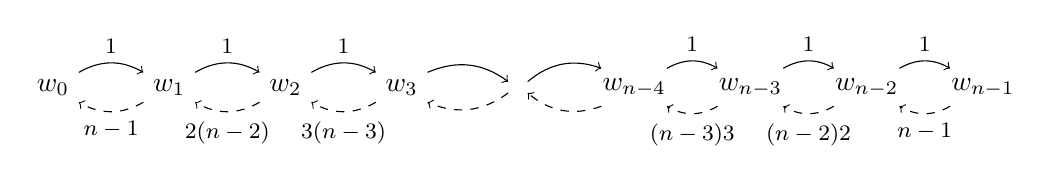
\begin{tikzpicture}[node distance = 4.2em]
     % the nodes
     \node (w0) {$w_0$};
     \node[right of = w0] (w1) {$w_1$};
     \node[right of = w1] (w2) {$w_2$};
     \node[right of = w2] (w3) {$w_3$};
     \node[right of = w3] (dots) {$\dotso$};
     \node[right of = dots] (wn-4) {$w_{n-4}$};
     \node[right of = wn-4] (wn-3) {$w_{n-3}$};
     \node[right of = wn-3] (wn-2) {$w_{n-2}$};
     \node[right of = wn-2] (wn-1) {$w_{n-1}$};
     % the action of e
     \draw[->, bend left] (w0) to node[above] {\footnotesize $1$} (w1);
     \draw[->, bend left] (w1) to node[above] {\footnotesize $1$} (w2);
     \draw[->, bend left] (w2) to node[above] {\footnotesize $1$} (w3);
     \draw[->, bend left] (w3) to (dots);
     \draw[->, bend left] (dots) to (wn-4);
     \draw[->, bend left] (wn-4) to node[above] {\footnotesize $1$} (wn-3);
     \draw[->, bend left] (wn-3) to node[above] {\footnotesize $1$} (wn-2);
     \draw[->, bend left] (wn-2) to node[above] {\footnotesize $1$} (wn-1);
     % the action of f
     \draw[->, bend left, dashed] (wn-1) to node[below] {\footnotesize $n-1$} (wn-2);
     \draw[->, bend left, dashed] (wn-2) to node[below] {\footnotesize $(n-2)2$} (wn-3);
     \draw[->, bend left, dashed] (wn-3) to node[below] {\footnotesize $(n-3)3$} (wn-4);
     \draw[->, bend left, dashed] (wn-4) to (dots);
     \draw[->, bend left, dashed] (dots) to (w3);
     \draw[->, bend left, dashed] (w3) to node[below] {\footnotesize $3(n-3)$} (w2);
     \draw[->, bend left, dashed] (w2) to node[below] {\footnotesize $2(n-2)$} (w1);
     \draw[->, bend left, dashed] (w1) to node[below] {\footnotesize $n-1$} (w0);
    \end{tikzpicture}
   \end{center}
   The desired basis $v_1, \dotsc, v_n$ can now be defined as
   \[
    v_i \coloneqq \frac{w_{i-1}}{(i-1)!}
    \quad \text{for every $i = 1, \dotsc, n$}.
    \qedhere
   \]
 \end{enumerate}
\end{proof}


\begin{expls}
 \begin{enumerate}[leftmargin=*]
  \item
   The one-dimensional irreducible representation of $\sll_2(k)$ can be realized by $\sll_2(k)$ acting trivially on $k$ (or any one-dimensional vector space for that matter.)
  \item
   The two-dimensional irreducible representation of $\sll_2(k)$ can be realized as the natural representation of $\sll_2(k)$. The detailed calculations were already shown in Example~\ref{expl: natural representation of sl2}.
  \item
   Let $V = \sll_2(k)$ be the adjoint representation of $\sll_2(k)$. Because $\sll_2(k)$ is simple it follows that $V$ is irreducible and $V = V_{-2} \oplus V_0 \oplus V_2$ with $V_{-2} = k f$, $V_0 = k h$ and $V_2 = k e$.
 \end{enumerate}
\end{expls}


\begin{expl}
 The map
 \[
  \phi \colon \sll_2(k) \to \sll_3(k), \quad
  A \mapsto \begin{pmatrix} A & 0 \\ 0 & 0 \end{pmatrix}
 \]
 is a homomorphism of Lie algebras. Therefore $V \coloneqq \sll_3(k)$ can be made into a representation of $\sll_2(k)$ via
 \[
  \rho \colon \sll_2(k) \xlongrightarrow{\phi} \sll_3(k) \xlongrightarrow{\ad} \gl(\sll_3(k)) = \gl(V).
 \]
 Then $h$ acts on $V$ by $\ad(H)$ for
 \[
%   E \coloneqq
%   \begin{pmatrix}
%    0 & 1 & 0 \\
%    0 & 0 & 0 \\
%    0 & 0 & 0
%   \end{pmatrix},
%   \quad
  H \coloneqq \phi(h) =
  \begin{pmatrix}
   1 &  0 & 0 \\
   0 & -1 & 0 \\
   0 &  0 & 0
  \end{pmatrix},
%   \quad
%   F \coloneqq
%   \begin{pmatrix}
%    0 & 0 & 0 \\
%    1 & 0 & 0 \\
%    0 & 0 & 0
%   \end{pmatrix},
 \]

 Notice that this representation is not irreducible because $\phi(\sll_2(k))$ is a non-trivial subrepresentation. However, by Weyl’s theorem $V$ decomposes into the direct sum of irreducible subrepresentations and it will be shown how to do so:
 
 Let $e_{12}, e_{13}, e_{23}, e_{21}, e_{31}, e_{32}, h_1, h_2$ be the basis of $V$ with
 \[
  h_1 \coloneqq \diag(1, -1, 0) \quad\text{and}\quad h_2 \coloneqq \diag(0, 1, -1).
 \]
 Notice that
 \[
  [\diag(a_1, a_2, a_3), e_{ij}] = (a_i-a_j) e_{ij}
  \quad\text{for all $a_1, a_2, a_3 \in k$ and $i,j = 1, \dotsc, 3$}
 \]
 It follows that
 \[
  e_{21} \in V_{-2}, \quad
  e_{23}, e_{31} \in V_{-1}, \quad
  h_1, h_2 \in V_0, \quad
  e_{13}, e_{32} \in V_1, \quad
  e_{12} \in V_2.
 \]
 So $V = \bigoplus_{i \in \Z} V_i$ with dimensions
 \begin{equation}\label{eqn: dimensions of eigenspaces of sl3}
  \dim V_i =
  \begin{cases}
   1 & \text{if $i = -2, 2$}, \\
   2 & \text{if $i = -1, 0, 1$}, \\
   0 & \text{otherwise}.
  \end{cases}
 \end{equation}
 
 Suppose that $V = W^1 \oplus W^2$ for two four-dimensional irreducible subrepresentations $W^1$ and $W^2$. Then
 \[
  W^1 = W^1_{-3} \oplus W^1_{-1} \oplus W^1_1 \oplus W^1_3
  \quad\text{and}\quad
  W^2 = W^2_{-3} \oplus W^2_{-1} \oplus W^2_1 \oplus W^2_3.
 \]
 and it follows that
 \[
  V = \underbrace{W^1_{-3} \oplus W^2_{-3}}_{= V_{-3}} \oplus
      \underbrace{W^1_{-1} \oplus W^2_{-1}}_{= V_{-1}} \oplus
      \underbrace{W^1_1 \oplus W^2_1}_{= V_{1}}  \oplus
      \underbrace{W^1_3 \oplus W^2_3}_{= V_{3}},
 \]
 contradicting \eqref{eqn: dimensions of eigenspaces of sl3}.
 
 To emphasize the approach which will be taken suppose that there exists a decomposition $V = W^{1,1} \oplus W^{1,2} \oplus W^{1,3} \oplus W^{2,1} \oplus W^{3,1}$ into irreducible subrepresentations with $\dim W^{1,1} = \dim W^{1,2} = \dim W^{1,3} = 1$, $\dim W^{2,1} = 2$ and $\dim W^{3,1} = 3$. Then
 \begin{align*}
  V
  &= W^{1,1} \oplus W^{1,2} \oplus W^{1,3} \oplus W^{2,1} \oplus W^{3,1} \\
  &= \underbrace{W^{3,1}_{-2}}_{= V_{-2}} \oplus
     \underbrace{W^{2,1}_{-1}}_{= V_{-1}} \oplus
     \underbrace{W^{1,1}_0 \oplus W^{1,2}_0 \oplus W^{1,3}_0 \oplus W^{3,1}_0}_{= V_0} \oplus
     \underbrace{W^{2,1}_1}_{= V_1} \oplus
     \underbrace{W^{3,1}_1}_{= V_2},
 \end{align*}
 also contradicting \eqref{eqn: dimensions of eigenspaces of sl3}.
 
 The above observations can easily be generalized: Let $V = \bigoplus_{d \geq 0} \bigoplus_{j=1}^{\nu_d} W^{d,j}$ be a decomposition into irreducible subrepresentations with $W^{d,j}$ being $d$-dimensional. As in the previous examples it follows that $V_i = \bigoplus_{p \in \N, d=|i|+1+2p} \bigoplus_{j=1}^{\nu_d} W^{d,j}_i$ for every $i \in \Z$ and therefore $\dim V_i = \sum_{p \in \N, d=|i|+1+2p} \nu_d$. Hence
 \[
  \nu_d \coloneqq \dim V_{d-1} - V_{d+1}
  \quad\text{for every $d \geq 1$}.
 \]
 With this it follows from \eqref{eqn: dimensions of eigenspaces of sl3} that $\nu_1 = 1$, $\nu_2 = 2$ and $\nu_3 = 1$.
 
 The three-dimensional irreducible subrepresentation is given by
 \[
  W^{3,1} \coloneqq \phi(\sll_2(k)) = \vspan_k(e_{12}, h_1, e_{21})
 \]
 The two two-dimensional irreducible subrepresentations $W^{2,1}$ and $W^{2,2}$ must satisfy
 \[
  W^{2,1} \oplus W^{2,2} = V_{-1} \oplus V_1 = \vspan_k(e_{23}, e_{31}, e_{13}, e_{32}).
 \]
 They then can be choosen as $W^{2,1} \coloneqq \vspan_k(e_{23}, e_{13})$ and $W^{2,2} \coloneqq \vspan_k(e_{31}, e_{32})$. That these are indeed subrepresentations follows from direct calculation. To find the one-dimensional irreducible subrepresentation notice that
 \begin{gather*}
  e.h_1 = -2e_{12}, \quad h.h_1 = 0, \quad f.h_1 = 2e_{21},
 \shortintertext{and}
  e.h_2 = e_{12}, \quad h.h_2 = 0, \quad f.h_2 = -e_{21}.
 \end{gather*}
 Hence $\sll_2(k)$ acts trivially on the one-dimensional linear subspace $W^{1,1} \coloneqq k (h_1 + 2h_2)$, which is why it is a subrepresentation.
\end{expl}


\begin{thrm}\label{thrm: finite dimensional representations of sl2}
 Let $V$ be a finite dimensional representation of $\sll_2(k)$.
 \begin{enumerate}[leftmargin=*]
  \item
   $V = \bigoplus_{d \geq 1} \bigoplus_{j=1}^{\nu_d} W^{d,j}$ where $W^{d,j} \subseteq V$ is an irreducible $d$-dimensional subrepresentation for all $d \geq 1$ and $j = 1, \dotsc, \nu_d$.
  \item
   $V = \bigoplus_{i \in \Z} V_i$ with
   \begin{equation}\label{eqn: eigenspace of a finite dimensional representation}
    V_i = \bigoplus_{\substack{p \in \N \\ d = |i|+1+2p}} \bigoplus_{j=1}^{\nu_d} W^{d,j}_i
    \quad \text{for every $i \in \Z$}
   \end{equation}
   and $\dim V_i = \sum_{p \in \N, d = |i|+1+2p} \nu_d$ for every $i \in \Z$.
  \item 
   The numbers $\nu_d$ for $d \geq 1$ are unique with $\nu_d = \dim V_{d-1} - \dim V_{d+1}$ for every $d \geq 1$.
  \item
   $\dim V_i = \dim V_{-i}$ for every $i \in \Z$.
 \end{enumerate}
\end{thrm}
\begin{proof}
 That $V$ decomposes into the direct sum of irreducible subrepresentations follows directly from Weyl’s theorem. From the classification of finite dimensional irreducible representations of $\sll_2(k)$ it follows that
 \[
  W^{d,j}
  = W^{d,j}_{-d+1} \oplus W^{d,j}_{-d+3} \oplus \dotsb \oplus W^{d,j}_{d-3} \oplus W^{d,j}_{d-1}
  = \bigoplus_{p=0}^{d-1} W^{d,j}_{-d+1+2p}
 \]
 for every $d \geq 1$ and $j = 1, \dotsc, \nu_d$. It follows that
 \[
  V
  = \bigoplus_{d \geq 1} \bigoplus_{j=1}^{\nu_d} W^{d,j}
  = \bigoplus_{d \geq 1} \bigoplus_{j=1}^{\nu_d} \bigoplus_{p=0}^{d-1} W^{d,j}_{-d+1+2p}.
 \]
 This shows that $V_i = \bigoplus_{i \in \Z} V_i$. Formula \eqref{eqn: eigenspace of a finite dimensional representation} follows from reordering the summands. It follows that
 \[
  \dim V_i
  = \dim \bigoplus_{\substack{p \in \N \\ d = |i|+1+2p}} \bigoplus_{j=1}^{\nu_d} W^{d,j}_i
  = \sum_{\substack{p \in \N \\ d = |i|+1+2p}} \sum_{j=1}^{\nu_d} \underbrace{\dim W^{d,j}_i}_{=1}
  = \sum_{\substack{p \in \N \\ d = |i|+1+2p}} \nu_d.
 \]
 As a direct consequence it follows that $\dim V_i = \dim V_{-i}$ for every $i \in \Z$ and
 \[
  \dim V_{i-1} - \dim V_{i+1}
  = \sum_{\substack{p \in \N \\ d = i+2p}} \nu_d - \sum_{\substack{p \in \N \\ d = i+2+2p}} \nu_d
  = \nu_i
  \quad\text{for every $i \geq 1$}.
 \qedhere
 \]
\end{proof}


\begin{expl}\label{expl: decomposition of the tensor product of 4 and 5}
 For every $n \geq 1$ let $V^{(n)}$ be the $n$-dimensional irreducible representation of $V$ and abbreviate $V \coloneqq V^{(4)}$ and $W \coloneqq V^{(5)}$. Then
 \begin{equation}\label{eqn: decomposition of 4 tensor 5}
  V \otimes W \cong V^{(8)} \otimes V^{(6)} \otimes V^{(4)} \otimes V^{(2)}.
 \end{equation}
 To see this notice that for $i,j \in \Z$ with $v \in V_\lambda$ and $w \in W_\lambda$ it follows that
 \[
  h.(v \otimes w)
  = (h.v) \otimes w + v \otimes (h.w)
  = iv \otimes w + jv \otimes w
  = (i+j) v \otimes w
 \]
 and therefore $V_i \otimes W_j \subseteq (V \otimes W)_{i+j}$. It follows that
 \begin{align*}
  (V \otimes W)_{-7}
  &= V_{-3} \otimes W_{-4}, \\
  (V \otimes W)_{-5}
  &= (V_{-3} \otimes W_{-2}) \oplus (V_{-1} \oplus W_{-4}), \\
  (V \otimes W)_{-3}
  &= (V_{-3} \otimes W_0) \oplus (V_{-1} \otimes W_{-2}) \oplus (V_1 \otimes W_{-4}), \\
  (V \otimes W)_{-1}
  &= (V_{-3} \otimes W_2) \oplus (V_{-1} \otimes W_0) \oplus (V_1 \otimes W_{-2}) \oplus (V_3 \otimes W_{-4}), \\
  (V \otimes W)_1
  &= (V_{-3} \otimes W_4) \oplus (V_{-1} \otimes W_2) \oplus (V_1 \otimes W_0) \oplus (V_3 \otimes W_{-2}), \\
  (V \otimes W)_3
  &= (V_{-1} \otimes W_4) \oplus (V_1 \otimes W_2) \oplus (V_3 \otimes W_0) \\
  (V \otimes W)_5
  &= (V_1 \otimes W_4) \oplus (V_3 \otimes W_2) \\
  (V \otimes W)_7
  &= V_3 \otimes W_4.
 \end{align*}
 with each of the summands being one-dimensional. It follows that
 \[
  \begin{array}{crrrrrrrrc}
   i \in \Z             & -7 & -5 & -3 & -1 & 1 & 3 & 5 & 7 & \text{otherwise} \\
   \hline
   \dim (V \otimes W)_i &  1 &  2 &  3 &  4 & 4 & 3 & 2 & 1 & 0
  \end{array}
 \]
 Formula \eqref{eqn: decomposition of 4 tensor 5} follows from this by Theorem \ref{thrm: finite dimensional representations of sl2}.
\end{expl}


\begin{rem}
 Example~\ref{expl: decomposition of the tensor product of 4 and 5} can be generalized to
 \[
  V^{(n)} \otimes V^{(m)}
  \cong V^{(n+m-1)} \oplus V^{(n+m-3)} \oplus \dotsb \oplus V^{(n-m+3)} \oplus V^{(n-m+1)}
 \]
 where $n, m \geq 1$ with $n \geq m$.
\end{rem}


% TODO: Remark about point diagrams


% TODO: Remark about dual representation for nice basis


% TODO: Decomposition of the tensor product












